% meta.concepts: 2D vector
% meta.tags: realistic
% acknowledge: Organic Navigation photo
% inspiration: Beer, Johnston, and Mazurek (Problem 2.41, 12th Edition)

A disabled lift has the loading shown at point $B$ and is being supported by a cable pulling along $BC$.  Find the required tension in cable $BC$ so that the resultant of the three forces at point $B$ is directed along the lift boom (i.e. member $AB$).

\begin{figure}[ht!]
  \centering
  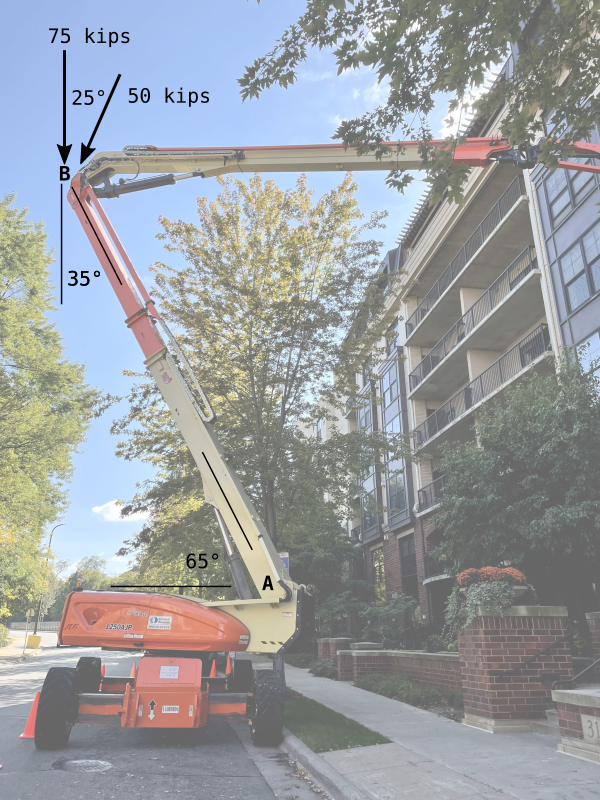
\includegraphics[width=3.0in]{fig.png}
\end{figure}

